\begin{frame}{Scientific context}
	\begin{minipage}{0.75\linewidth}
		\textbf{Context :} Create real-time digital twins of an organ (e.g. liver).
	\end{minipage}
	\begin{minipage}{0.21\linewidth}
		\vspace{-20pt}
		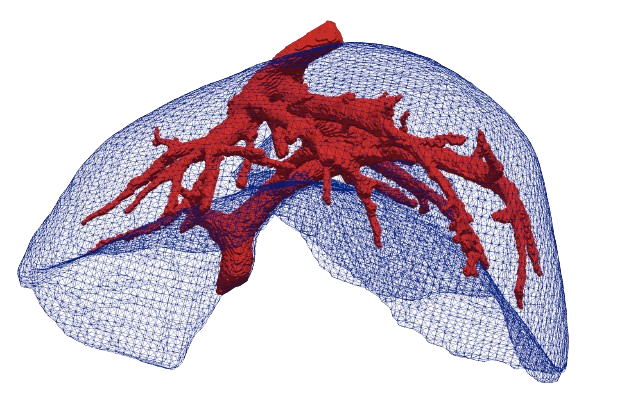
\includegraphics[width=\linewidth]{images/intro/liver.png}
	\end{minipage}
	
	\vspace{5pt}
	\textbf{Objective :} Develop an hybrid \fcolorbox{red}{white}{finite element} / \fcolorbox{orange}{white}{neural network} method.
	
	\vspace{1pt}
	\small
	\hspace{130pt} \begin{minipage}{0.14\linewidth}
		\textcolor{red}{accurate}
	\end{minipage} \hspace{8pt} \begin{minipage}{0.3\linewidth}
		\textcolor{orange}{quick + parameterized}
	\end{minipage}

	\normalsize
	\vspace{5pt}
	\textbf{\filledstar Parametric elliptic convection/diffusion PDE :}
	For one or several  $\bm{\mu}\in \mathcal{M}$, find $u: \Omega\to \mathbb{R}$ such that
	\begin{equation}
		\label{eq:ob_pde}
		\mathcal{L}\big(u\,;\bm{x},\bm{\mu}\big) = f(\bm{x},\bm{\mu}),
		\tag{$\mathcal{P}$}
	\end{equation}
	where $\mathcal{L}$ is the parametric differential operator defined  by
	\begin{equation*}
		\mathcal{L}(\cdot;\bm{x},\bm{\mu}) : u \mapsto R(\bm{x},\bm{\mu}) u + C(\bm{\mu}) \cdot \nabla u - \frac{1}{\text{Pe}} \nabla \cdot (D(\bm{x},\bm{\mu}) \nabla u),
	\end{equation*}
	and some Dirichlet, Neumann or Robin BC (which can also depend on $\bm{\mu}$).
\end{frame}

\begin{frame}{Pipeline of the Enriched FEM}
	Enriched FEM = Combination of 2 standard methods
	\begin{itemize}
		\item \textbf{PINNs} : Physics Informed Neural Networks \quad \refappendix{frame:pinns}
		\item \textbf{FEMs} : Finite Element Methods \quad \refappendix{frame:fems}
	\end{itemize}

	\begin{figure}[!ht]
		\centering
		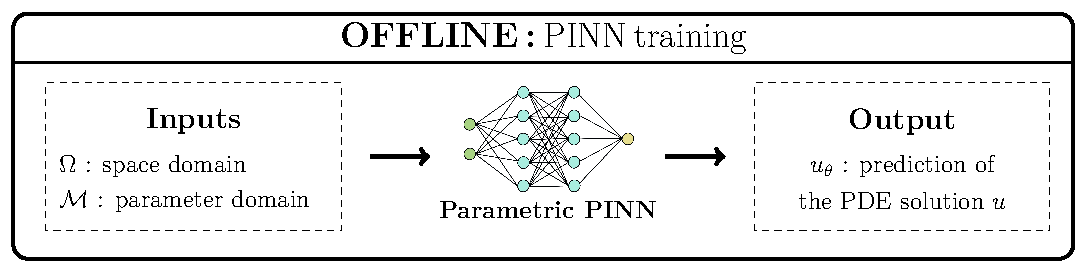
\includegraphics[width=0.7\linewidth]{images/intro/pipeline/offline.pdf}

		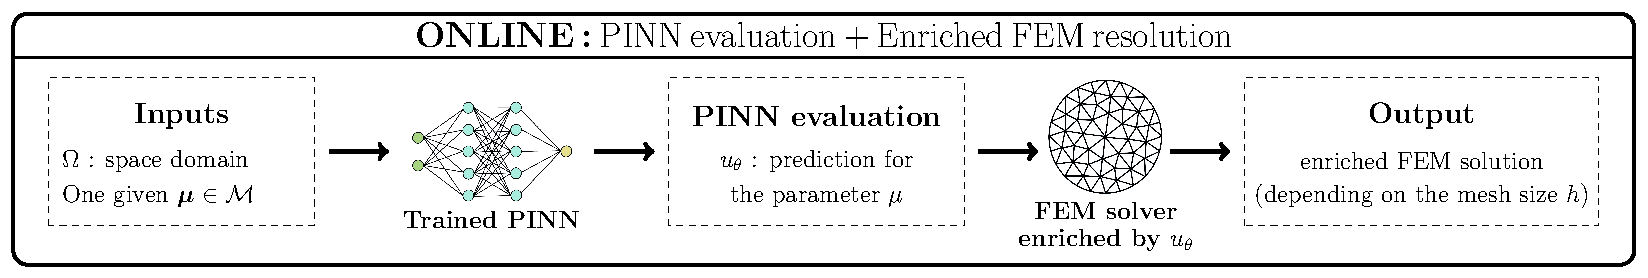
\includegraphics[width=\linewidth]{images/intro/pipeline/online.pdf}
	\end{figure}

	\textbf{Remark :} The PINN prediction enriched Finite element approximation spaces.
\end{frame}